\documentclass{article}
\usepackage[utf8]{inputenc}
\usepackage[T1]{fontenc}
\usepackage{geometry}
\geometry{
    a4paper,
    left=2.5cm,
    right=2.5cm,
    top=2.5cm,
    bottom=2.5cm
}
\usepackage{graphicx}
\usepackage{float}
\usepackage{hyperref}
\usepackage[english]{babel}
\usepackage{amsmath}
\usepackage{amssymb}
\usepackage{array}
\usepackage{booktabs}
\usepackage{caption}
\usepackage{subcaption}
\usepackage{enumitem}
\usepackage{fancyhdr}
\usepackage{titlesec}
\usepackage{url}
\usepackage{textcomp}
\usepackage{xcolor}
\usepackage{listings}
\usepackage{multirow}
\usepackage{longtable}
\usepackage{tabularx}
\usepackage{times}

% Set up page style
\pagestyle{fancy}
\fancyhf{}
\rfoot{\thepage}
\renewcommand{\headrulewidth}{0pt}

% Title formatting
\titleformat{\chapter}[display]{\normalfont\bfseries}{\chaptertitle\thechapter}{0pt}{\Huge}
\titlespacing*{\chapter}{0pt}{50pt}{40pt}

% Document info
\title{Template Document}
\author{Academic Support Agent}
\date{\today}

\begin{document}
\maketitle

% Koferenznamen festlegen (Fu zeile)
\conference{Vorgestellt auf der \enquote{Konferenztitel}, Stadt, Land, Jahr}

\maketitle\vspace{-1em}

%%% Begin of Multicols-Enviroment
\begin{multicols}{3}

\section{Einleitung}

\begin{block}{Sinn und Zweck einer Posterpr sentation:}
	\begin{itemize}
		\item Darstellung der wichtigsten Ergebnisse der Arbeit
		\item Interesse f r die Arbeit/den Bericht zu wecken
		\item Ziel: lehrreich und unterhaltsam zugleich
	\end{itemize}
\end{block}

\begin{block}{Vorteile von \LaTeX\ mit der \textsc{sciposter}-Klasse:}
	\begin{itemize}
		\item sehr einfach, wenn die Arbeit bereits in \LaTeX\ erstellt wurde
		\item verschiedene Darstellungsvarianten zur Auswahl
		\item Folieninhalte k nnen unter Nutzung des \emph{beamerarticle}-Pakets einfach  bernommen werden
	\end{itemize}
\end{block}

\section{Hauptteil}

\subsection{Gleichungen}

\begin{block}{Satz des Pythagoras:}
	\begin{equation}
		a^2 + b^2 = c^2 \label{eq:pythogoras}
	\end{equation}
\end{block}

\begin{block}{Es folgt, dass:}
	\begin{align}
		a^2 &= c^2 - b^2 \\
		b^2 &= c^2 - a^2
	\end{align} 	
\end{block}
	
\subsection{Tabellen}

\begin{table}
	\caption{Beispieltabelle}
	\label{tab:beispiel}
	\centering
		\begin{tabular}{cc}
			\toprule
			Variable & Bedeutung \\
			\midrule
			$t$ & Zeit \\
			$U$ & Spannung \\
			\bottomrule
		\end{tabular}
\end{table}

\subsection{Abbildungen}

\begin{figure}
	\centering
		\includegraphics[width=0.7\columnwidth]{logos/unilogo}
	\caption{Altes Logo der Universit t}
	\label{fig:unilogo}
\end{figure}

\begin{figure}
	\centering
		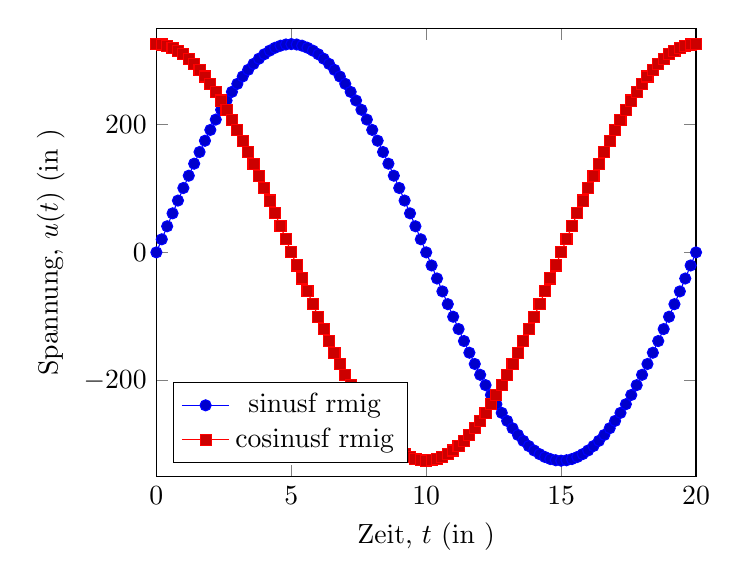
\begin{tikzpicture}
			\begin{axis}[
				xlabel={Zeit, $t$ (in \si{\milli\second})},
				ylabel={Spannung, $u(t)$ (in \si{\volt})},
				xmin=0,xmax=20,
				ymin=-350,ymax=350,
				legend pos=south west,
				% Beispiel zum direkten Einf gen von Formeln
				]
				\addplot+[
					domain=0:20,
					samples=101,
				] {sin(deg(x*2*pi/20))*sqrt(2)*230};
				\addlegendentry{sinusf rmig};
				\addplot+[
					domain=0:20,
					samples=101,
				] {cos(deg(x*2*pi/20))*sqrt(2)*230};
				\addlegendentry{cosinusf rmig};
			\end{axis}
		\end{tikzpicture}
	\caption{Harmonischer Zeitverlauf einer Spannung mit einer Frequenz von \SI{50}{\hertz} und einem Effektivwert von \SI{230}{\volt}}
	\label{fig:u_t_sinus}
\end{figure}

\begin{block}{Zitate:}
	\begin{itemize}
		\item Kurzzitate wie~~\cite{lanze:manuskript} k nnen benutzt werden
		\item Leser kann die Nummer im Literaturverzeichnis nachschlagen
		\item Alternative: Vollzitate
	\end{itemize}
\end{block}
\begin{block}{Beispiel f r ein Vollzitat:}
	\small\fullcite{hering:berichte}
\end{block}

\section{Zusammenfassung und Ausblick}

\begin{block}{Zusammenfassung:}
	\begin{itemize}
		\item Kurzfassung der wichtigsten Ergebnisse
		\item Aufzeigen nicht gel ster Probleme und offener Fragen
		\item eventuell Ausblick auf weitere geplante Forschungsarbeiten
	\end{itemize}
\end{block}

\begin{block}{Ausblick:}
	\begin{itemize}
		\item Welche Forschungsfragen sind noch offen?
		\item Wo w rde man weitermachen, wenn man mehr Zeit h tte?
	\end{itemize}
\end{block}	

\begin{block}{Download von \url{http://www.musteradresse.de/} or via QR Code:}
	\begin{center}
		\qrcode[height=0.7\columnwidth]{http://www.musteradresse.de/}
	\end{center}
\end{block}

\end{multicols}

% Literaturverzeichnis
\printbibliography
\end{document}